\section{Introduzione}

Per caratterizzare meccanicamente la cellula e le sue prprietà viscoelastiche è necessario avere un modello descrittivo del comportamento.

Viene quindi considerato un modello a parametri concentrati costituito da uno smorzatore in serie ad un ramo dato dal paralello di un corpo di Maxwell e una rigidezza elastica.



\section{Background}

Le proprietà cellulari sono il principale motivo di indagine e ricerca. Tra queste le proprietà meccaniche sono utili biomarker \cite{di_carlo_mechanical_2012}. 

La deformabilità e le proprietà viscoeleastiche sono utili indicatori di cambiamenti citoscheletrici e dello stato cellulare .  

Ne sono esempi l'aumento di rigidezza nei globuli rossi affetti da sferocitosi \cite{lee_biomechanics_2007,suresh_connections_2005} e l'aumento di deformabilità nella cellule cancerogene \cite{mierke_viscoelasticity_2021}.

Tali proprietà meccaniche possono essere misurate con differenti tecniche quali microscopio a forza atomica, trappole ottiche, microreometro a biglia magnetica e l'aspirazione con micropipette \cite{ethier_introductory_nodate}.

In questo report viene posta l'attenzione su un microreometro a biglie magnetiche e il modello di cellula per stimarne le proprietà viscoelastiche.


\begin{figure*}[t!]
	\begin{subfigure}{0.5\linewidth}
		\centering
		\footnotesize{
			\def\svgwidth{0.9\linewidth}
			\input{mechanic_model.pdf_tex}}
		\caption{}
		\label{fig:mechanical}
	\end{subfigure}\hfill
	\begin{subfigure}{0.5\linewidth}
		\centering
		\footnotesize{
			\def\svgwidth{0.9\linewidth}
			\input{creep_response.pdf_tex}}
		\caption{}
		\label{fig:mechanical1}
	\end{subfigure}\hfill
	\caption{Modello utilizzato per la descrizione del comportamento cellulare (a) e comportamento meccanico del modello (b) dove è possibile identificare diversi fasi quali fast elastic response (I), relaxation regime (II) e flow regime (III).}
\end{figure*}
\begin{figure}[b!]
	\centering
	\footnotesize{
	 \def\svgwidth{\linewidth}
	 \input{rheometer.pdf_tex}}
	\caption{}
	\label{fig:system}
\end{figure}



\subsection{Microreometro a biglia magnetica}

Il microreometro è un dispositivo utilizzato nella micro reologia per caratterizzare le proprietà reologiche di un mezzo quali la viscosità o le tracce di flusso. Tali dispositivi si misura si dividono in attivi e passivi a seconda che sfruttano l'energia termica o forze esterne applicate per movimentare la particella.

In questo report viene analizzato un microreometro a biglie magnetiche. Tali biglie paramagnetiche di 4.5 $\mu m$ di diametro sono legate al citoscheletro cellulare tramite la connessione tra le integrine di membrana e la fibronectina di cui sono ricoperte le biglie. L'integrina di membrana è connessa direttamente al citosceheltro quindi la misura dello spostamento della biglia fornisce informazioni sulla meccanica cellulare.

La presenza di un campo magnetico controllato applica una forza sulla miglia e misurandone lo spostamento è possibile caratterizzarne alcune proprietà viscoelastiche \cite{bausch_local_1998} fissando un modello viscoelastico di cellula.

Il comportamento osservato è rappresentato in \cref{fig:mechanical1} ed è possibile distinguere tre fasi principali. Come viene applicata la forza è c'è un primo spostamento della biglia (fase I) identificato come risposta elastica veloce. La prima fase è seguita dal regime di rilassamenti (fase II) e infine la regime di flusso, dove si verifica un progressivo scivolamento.

Considerando la seguente descrizione del modello è possibile stimarne sperimentalmente tre parametri quali l'ampiezza della prima fase $1\over k_1+k_0$, la costante di tempo dell'andamento esponenziale della fase II $\tau=\frac{\gamma_{1}\left(k_{0}+k_{1}\right)}{k_{0} k_{1}}$ e il parametro $\gamma_0$ identificativo dell'ampiezza della fase III. 

Tali valori, stimati da \cite{bausch_local_1998}, verranno utilizzati per implementare una soluzione numerica del modello all'interno dell'ambiente Matlab.



\subsection{Modello meccanico}

\begin{figure*}[t!]
	\begin{subfigure}{0.5\linewidth}
		\centering
		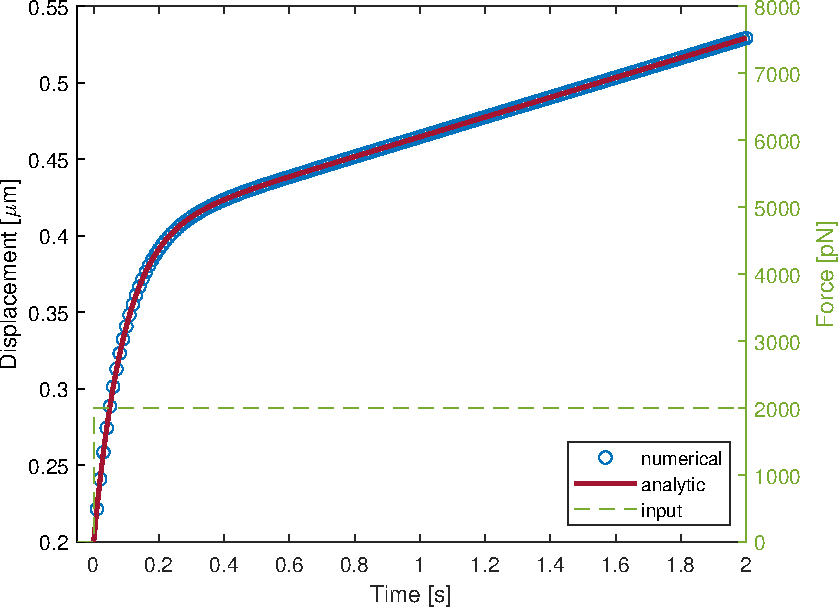
\includegraphics[width=0.95\linewidth]{../code/figs/step}
		\caption{}
		\label{fig:step}
	\end{subfigure}\hfill
	\begin{subfigure}{0.5\linewidth}
		\centering
		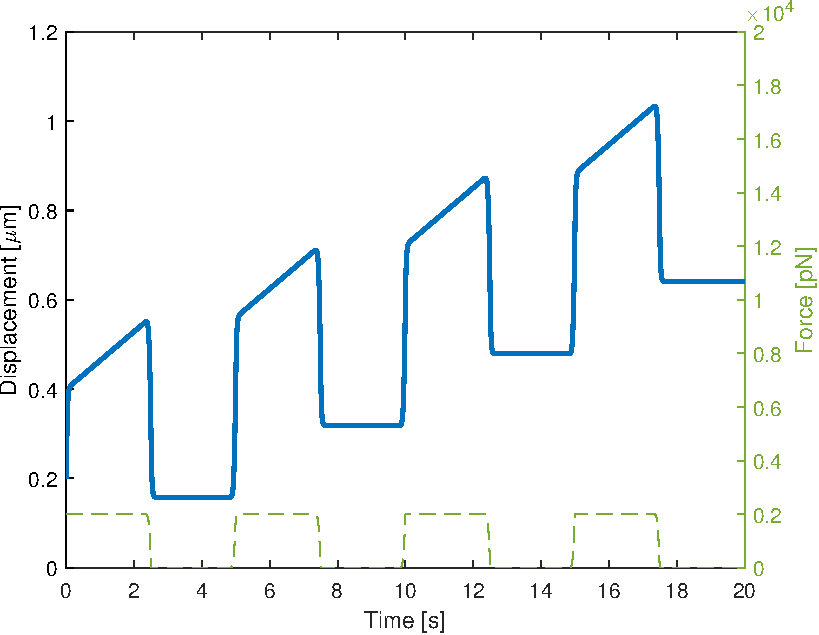
\includegraphics[width=0.95\linewidth]{../code/figs/square}
		\caption{}
		\label{fig:square}
	\end{subfigure}\hfill
	\caption{Risposta del sistema ad ingresso a gradino (a) e ad onda quadra con periodo di 5s (b).}
\end{figure*}
Tali curve sono analizzate sulla base di un modello descritto da una serie di uno smorzato (a seguire indicato come Dashpot) e di un corpo Zener, noto anche come corpo Kelvin, descritto da un parallelo di una ramo descritto da una rigidezza elastica e un secondo ramo descritto dalla serie di uno smorzato e una rigidezza. Tale modello è rappresentato in \cref{fig:mechanical}.

La descrizione meccanica di tale segue dal fatto che lo spostamento risultante sarà proprio la somma del dashpot $\gamma_0$ (D) e del corpo Zener (Z).

\begin{equation}
	{x}(t)={x}_{D}(t)+{x}_{z}(t)
\end{equation}

E quindi derivando vale ancora:

\begin{equation}
	\dot{x}(t)=\dot{x}_{D}(t)+\dot{x}_{z}(t)
\end{equation}

Chiaramente la forza applicata sarà la stessa su entrambi.

Per (D) è nota la relazione dello smorzatore da cui possiamo ricavare la velocità come:

\begin{equation}
	\dot{x}_D={F\over \gamma_0}
\end{equation}


Per il corpo Zener la forza si distribuisce sul ramo elastico e sul ramo dove è presente un corpo Maxwell (molla e smorzatore). 

\begin{equation}
	F(t)=F_{\text {Maxwell }}(t)+F_{\text {Ko }}(t)
\end{equation}
 
Dove la forza applicata sul corpo di Maxwell è proprio la differenza tra quella totale applicata e quella del ramo elastico $k_0 x_Z(t)$.

Ovvero per il corpo Maxwell, derivando lo spostamento, si ottiene: 

\begin{equation}
	\dot{x}_Z(t)={\dot F\over k_1}+{F\over \eta_0}
\end{equation} 

E quindi complessivamente per il corpo Zener vale:

\begin{equation}
	\dot{x}_Z(t)={\dot F(t)-k_0\dot x(t) \over k_1}+{F(t)-k_0 x(t)\over \eta_0}
	\label{eq:zener}
\end{equation} 


In conclusione, lo spostamento sarà dato dalla somma dei due spostamenti che possono essere ricavati risolvendo le due equazioni differenziali per un dato ingresso e condizione iniziale.

\section{Risultati}

\begin{figure*}[t!]
\begin{lstlisting}[language=matlab]
	function dydt=zener_displacement(t,y,parameters,tspan,flag)
		k_0=parameters(1);
		k_1=parameters(2);
		gamma_0=parameters(3);
		gamma_1=parameters(4);
		F_bar=parameters(5);
		switch flag
			case 'square'
				[F, dF]=force(t,tspan);
				dydt=((F-k_0*y)/gamma_1 + (dF/k_1))*(1+k_0/k_1);
			case 'step'
				dydt=(-(k_0/gamma_1)*y+(F_bar/gamma_1))/(1+(k_0/k_1));
			case 'harmonic'
				omega=parameters(7);
				F=F_bar*(1+sin(omega*t));
				dF=F_bar*omega*cos(omega*t);
				dydt=((F-k_0*y)/gamma_1 + (dF/k_1))*(1+k_0/k_1);
		end
	end
\end{lstlisting}
\caption{Routine richiamata da \texttt{ode15s} per la soluzione dell'equazione differenziale per lo spostamento del corpo Zener}
\vspace{0.8cm}
\begin{lstlisting}[language=matlab]
	function dydt=dashpot_displacement(t,y,parameters,tspan,flag)
		gamma_0=parameters(3);
		gamma_1=parameters(4);
		F_bar=parameters(5);
		switch flag
			case 'square'
				[F, dF]=force(t,tspan);
				dydt=F/gamma_0;
			case 'step'
				dydt=F_bar/gamma_0;
			case 'harmonic'
				omega=parameters(7);
				F=F_bar*(1+sin(omega.*t));
				dF=F_bar*omega*cos(omega*t);
				dydt=F/gamma_0;
		end
	end	
\end{lstlisting}
\caption{Routine richiamata da \texttt{ode15s} per la soluzione dell'equazione differenziale per lo spostamento dello smorzatore}
\label{fig:routineode}
\end{figure*}



\subsection{Ingresso a gradino}

Per un ingresso a gradino, di ampiezza $\bar F$ otterremo per il dashpot l'equazione differenziale:

\begin{equation}
	\left\{\begin{array}{l}
		\dot{x}_D=\frac{\bar{F}}{\gamma_{o}} \quad t>0 \\
		x_{D}(0)=0
	\end{array}\right.
\end{equation}

Di soluzione analitica lineare nel tempo:

\begin{equation}
	x_D(t)={\bar F\over \gamma_0}t
\end{equation}

Tale risposta lineare è rappresentante della fase lineare osservata nelle misure sperimentali. 


Per il corpo Zener vale:

\begin{equation}
	\left\{\begin{array}{l}
		\dot{x}_{z}(t)\left(1+\frac{k_{o}}{k_{1}}\right)=-\frac{k_{o}}{\gamma_{1}} x_{z}+\frac{\bar{F}}{\gamma_{1}} \quad t>0 \\
		x_{z(0)}=\frac{\bar{F}}{k_{1}+k_{o}}
	\end{array}\right.
\end{equation}

Dove la condizione iniziale deriva dal fatto da considerare lo spostamento sullo smorzatore nullo all'instante iniziale e allora lo spostamento complessivo è legato alle sole rigidezze elastiche.

Considerando il tempo di rilassamento

\begin{equation}
\tau={\gamma_1}{k_1+k_1\over k_0k_1}
\end{equation} 


 
Si può riscrivere il problema come

\begin{equation}
		\left\{\begin{array}{l}
		\dot{x}_{z}(t) +{1\over \tau}x_Z(t)={\bar F\over k_0\tau} \quad t>0 \\
		x_{z(0)}=\frac{\bar{F}}{k_{1}+k_{o}}
	\end{array}\right.
\end{equation} 

Ovvero, tale problema di Cauchy presenta una soluzione del tipo:

\begin{equation}
x_z(t)=e-^{A(t)}\left[x_0+\int_{t_0}^{t} g(x) e^{A(t)}\right]
\end{equation}

Dove $A(t)$ è il termine legato alla soluzione dell'equazione omogenea, ovvero l'integrale del coefficiente che moltiplica $x_Z(t)$, mentre il termine $g(x)$ è legato all'equazione non omogenea.

Allora si ottiene:

\begin{equation}
	x_z(t)=e-^{t\over tau}\left[{F\over k_0+k_1}+{F\over k_0}e^{t\over \tau}-{F\over k_0}\right]
\end{equation}

Che può essere riscritta come:

\begin{equation}
	x_Z(t)={\bar F\over k_0}\left(1-{k_1\over k_0+k_1}e^{-{t\over \tau}}\right)
\end{equation}

Ovvero un'esponenziale che progressivamente tenderà a $\bar F\over k_0$. 

Inoltre, lo spostamento è raffigurato in \cref{fig:step} e \cref{fig:separati}.


Tale soluzione viene graficata in \cref{fig:step} e confrontata con la soluzione numerica ottenuta in Matlab.




\begin{figure*}[t!]
	\centering
	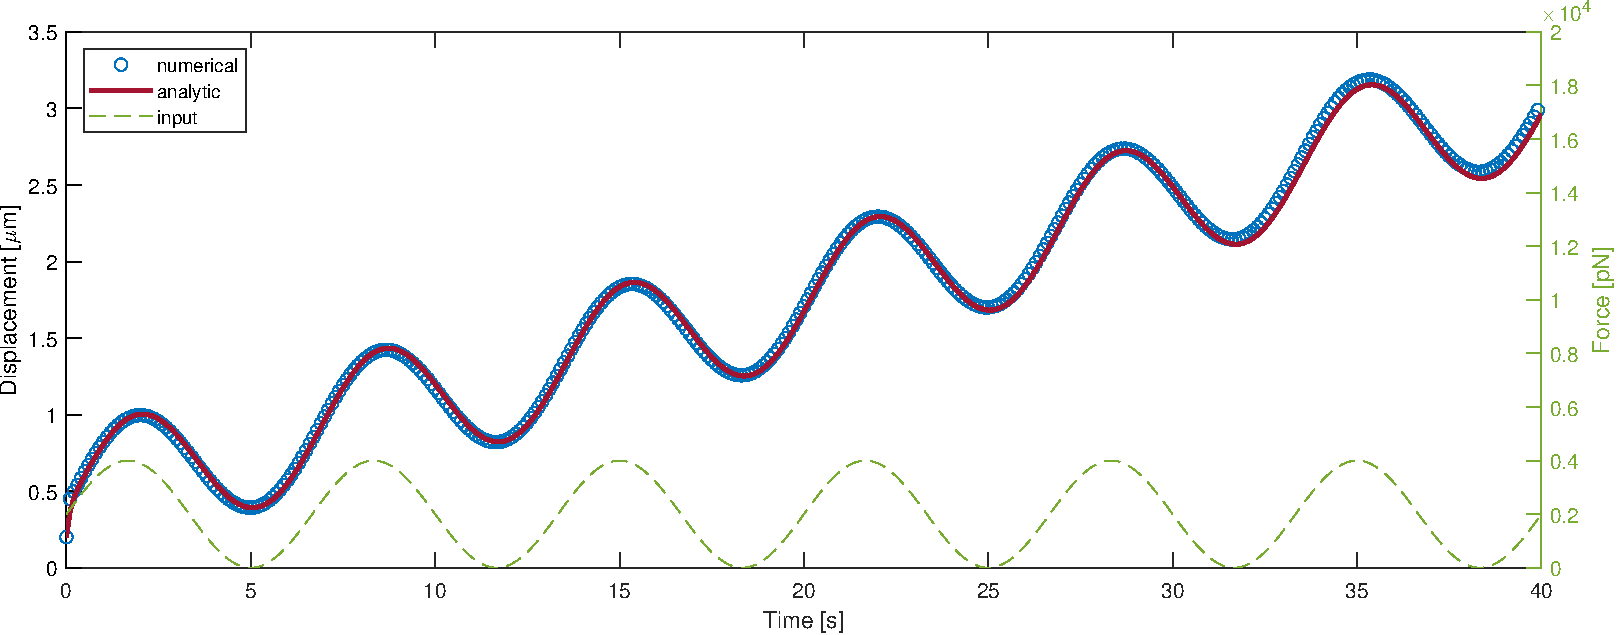
\includegraphics[width=0.95\linewidth]{../code/figs/harmoniclarge}
	\caption{Confronto tra il risultato analitico e il risultato numerico con ingresso sinusoidale a frequenza 0.15 Hz applicato per 40s.}
	\label{fig:harmoniclarge}
\end{figure*}

\begin{figure}[b!]
	\centering
	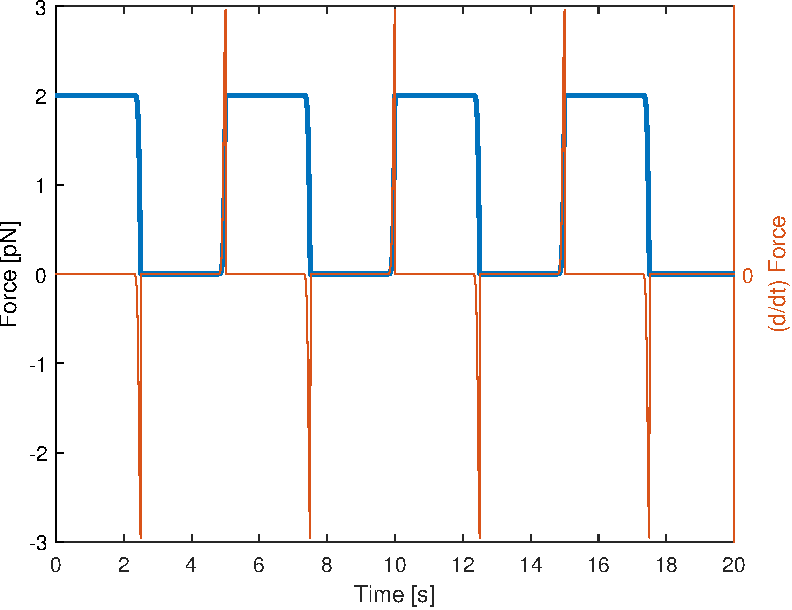
\includegraphics[width=0.95\linewidth]{../code/figs/square_regularized}
	\caption{Ingresso ad onda quadra regolarizzata dove le discontinuità sono state ammorbidite con un filtro gaussiano al fine di poter calcolare la derivata numerica. Tale segnale diventa l'ingresso per il modello meccanico.}
	\label{fig:squareregularized}
\end{figure}


\begin{figure*}[t!]
	\begin{lstlisting}[language=matlab]
		function [F, dF]=force(t_curr,t)	
		T_cyc=5;
		N_cyc=4;
		F=2000;
		freq=1/T_cyc;
		squareWave=F/2*(square(2*pi*freq*t,50)+1);
		squareWave(end)=0;
		squareWave_smooth=smoothdata(squareWave,'gaussian',(size(t)/N_cyc)*0.05);
		derivate=[0 diff(squareWave_smooth)];
		F=interp1(t,squareWave_smooth,t_curr);
		dF=interp1(t,derivate,t_curr);
		end
	\end{lstlisting}
	\caption{Routine per la generazione dell'onda quadra regolarizzata di ingresso. Viene inserita anche la funzione \texttt{interp1} per permette a \texttt{ode15s} di leggere il valore di forza a qualsiasi instante temporale ($\mathtt{t\_curr}$) e non solo sui campione dove è stato definito il segnale.}
	\label{fig:force}
\end{figure*}







\begin{figure*}[t!]
	\begin{subfigure}{0.33\linewidth}
		\centering
		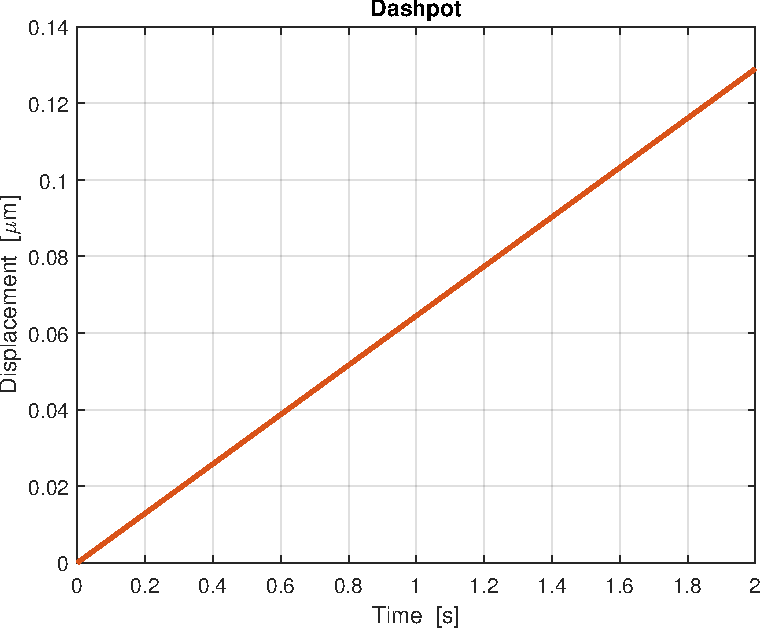
\includegraphics[width=0.95\linewidth]{../code/figs/step_dashpot_}
		\caption{}
	\end{subfigure}\hfill
	\begin{subfigure}{0.33\linewidth}
		\centering
		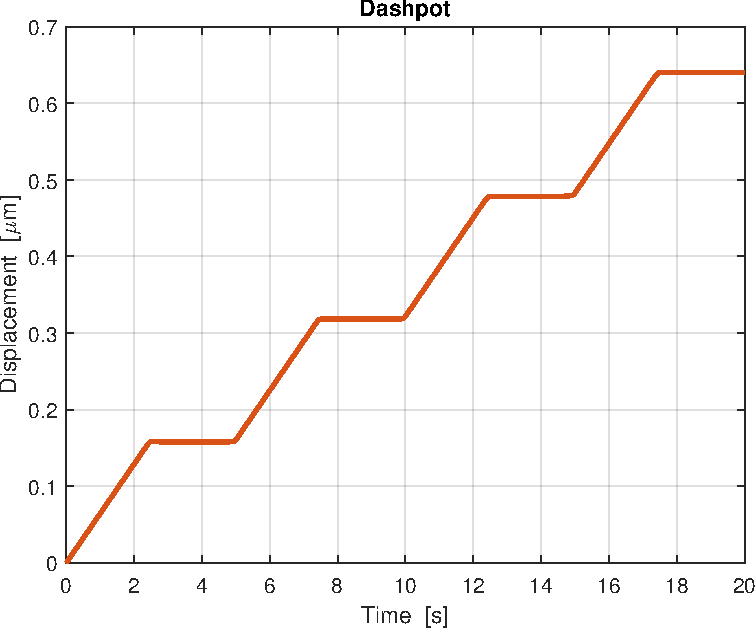
\includegraphics[width=0.95\linewidth]{../code/figs/square_dashpot_}
		\caption{}
	\end{subfigure}\hfill
	\begin{subfigure}{0.33\linewidth}
		\centering
		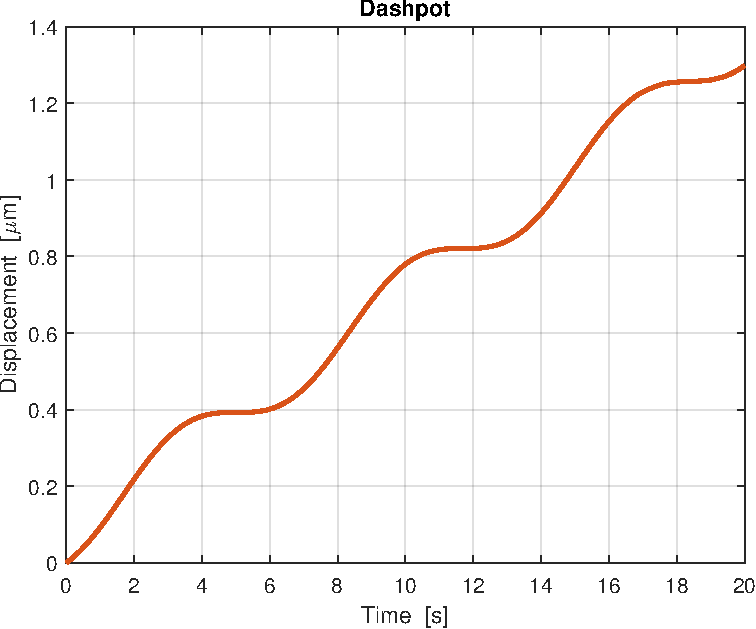
\includegraphics[width=0.95\linewidth]{../code/figs/harmonic_dashpot_}
		\caption{}
	\end{subfigure}\hfill
	\begin{subfigure}{0.33\linewidth}
		\centering
		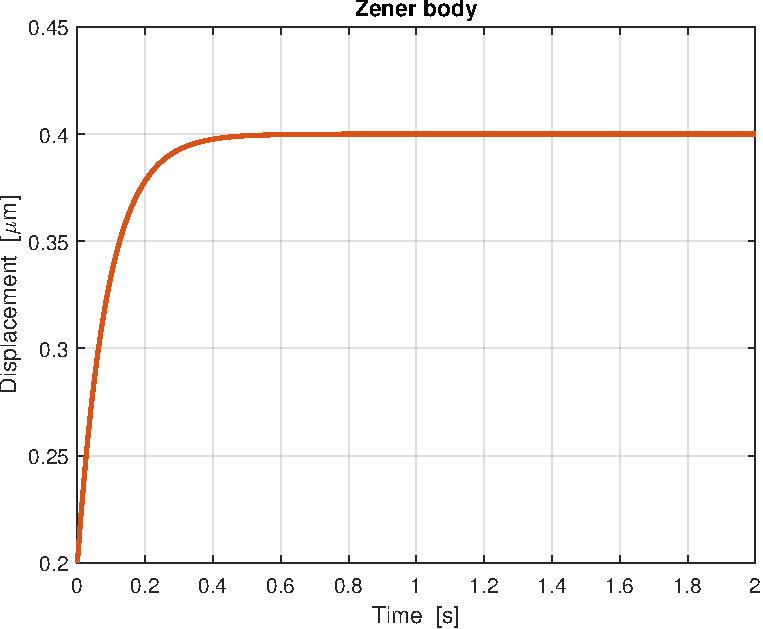
\includegraphics[width=0.95\linewidth]{../code/figs/step_zener_}
		\caption{}
	\end{subfigure}\hfill
	\begin{subfigure}{0.33\linewidth}
		\centering
		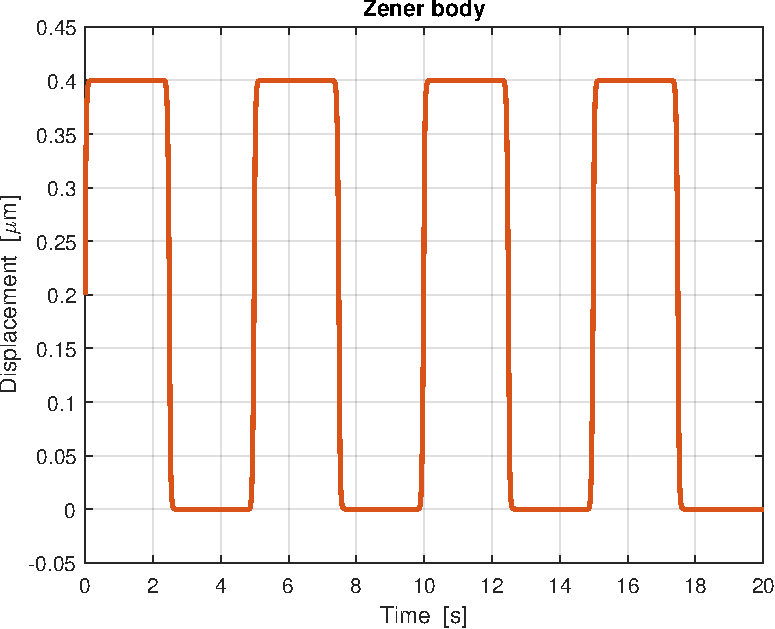
\includegraphics[width=0.95\linewidth]{../code/figs/square_zener_}
		\caption{}
	\end{subfigure}\hfill
	\begin{subfigure}{0.33\linewidth}
		\centering
		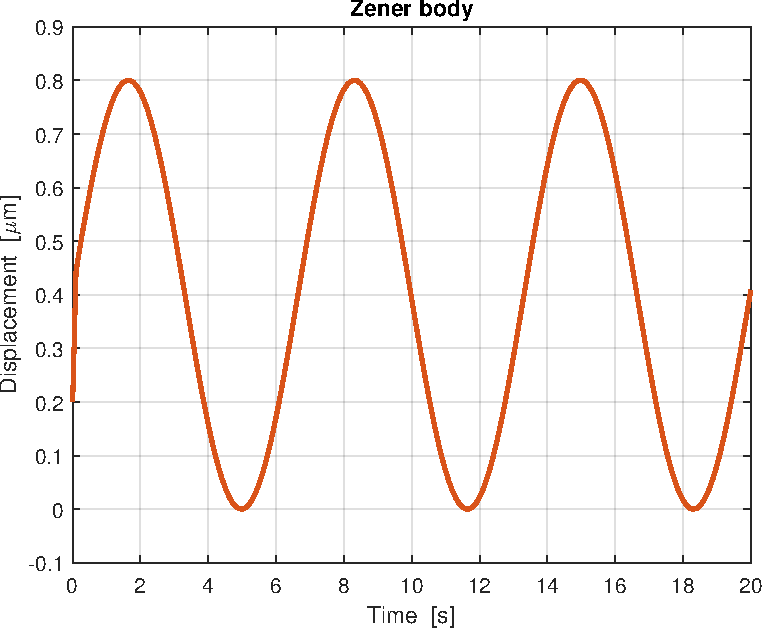
\includegraphics[width=0.95\linewidth]{../code/figs/harmonic_zener_}
		\caption{}
	\end{subfigure}\hfill
	\caption{Andamento dello spostamento dello smorzatore (sopra) e del corpo Zener (sotto) nel caso di ingresso a gradino (a,d); a onda quadra con periodo di 5s (b,e); sinusoide a frequenza 0.15 Hz (c,f).}
	\label{fig:separati}
\end{figure*}

\subsection{Soluzione numerica}

La soluzione numerica viene ottenuta in Matlab tramite $\mathtt{ode15s}$, un solutore proprietario per equazioni differenziali stiff.

La routine principale (\texttt{main.m}) permette di selezionare tramite la variabile $\mathtt{flag}$ il tipo di ingresso per la forza, scegliendo tra l'ingresso a gradino, un'onda quadra e una sinusoide, descritte più avanti.

Successivamente la routine setta un intervallo temporale appropriato e richiama $\mathtt{ode15s()}$ passandogli le funzioni dove sono definiti gli spostamenti (\cref{fig:routineode}) e poi viene graficata la loro somma.



\subsection{Ingresso a onda quadra}

Viene poi testato un ingresso ad onda quadra come utilizzato in \cite{bausch_local_1998}, con un periodo di 5s, un duty cicle del 50\% e un'ampiezza di 2000 pN, testata su un intervallo di 20s.

Tale ingresso viene implementato tramite la routine \texttt{force.m}, descritta in \cref{fig:force} avendo l'accortezza di ammorbidire il gradino per poterne fare la derivata numerica anche delle discontinuità e facendo in modo che $\mathtt{ode15s}$ possa richiederne il valore a qualsiasi instante, e non solo sui campione dove viene definita, tramite un'interpolazione.  Tale segnale è presente in \cref{fig:squareregularized}.

I risultati sono presenti in \cref{fig:square} e dalla scomposizione dei due segnali (\cref{fig:separati}) è possibile osservare come il dashpot presenta una componente lineare a tratti alla quale viene aggiunto il comportamento oscillatore del corpo Zener.



\subsection{Ingresso sinusoidale}

L'effetto oscillatorio è chiaramente molto presente se sollecitiamo il modello con un ingressi sinusoidale del tipo: 

\begin{equation}
	F(t)=\bar F\left(1+\sin (\omega t)\right)
\end{equation}

La soluzione analitica presenta sia una componente armonica che una esponenziale:

\begin{equation}
	\small{\begin{aligned}
	x(t)=\frac{F_{0}}{k_{0}}& \left[ 1-\frac{k_{1}}{k_{0}+k_{1}} e^{-t / \tau}\right.+ \\
		&\left.+\frac{\tau \omega\left(1-\frac{\gamma_{1}}{k_{1} \tau}\right)\left(e^{-t / \tau}-\cos \omega t\right)}{1+(\tau \omega)^{2}}\right.+\\
		&\left.+\frac{\left(1+\frac{\gamma_{1} \tau \omega^{2}}{k_{1}}\right) \sin \omega t}{1+(\tau \omega)^{2}}\right]
	\end{aligned}}
	\end{equation}

Tale soluzione viene confrontata con la soluzione numerica in \cref{fig:harmoniclarge}. 

Dai due spostamenti separati (\cref{fig:separati}) è possibile vede come entrambi hanno una componente armonica e mentre lo spostamento del corpo Zener è limitato il dashpot presenta una crescita lineare inviluppato da una sinusoide.


\section{Conclusioni}

Lo studio e la classificazione del comportamento meccanico di tali modelli permette di analizzarne i coefficienti e poter fittare dei dati sperimentali per ricavare le proprietà meccaniche cellulari.

Avvalersi di un solutore numerico permette di analizzare il modello meccanico anche per ingressi complessi e fortemente variabili nel tempo. 

Le costanti viscoelastiche stimate dal modello a parametri concentrati sono indicative delle proprietà dell'intera cellula, ma tali proprietà sono determinate in parte dalle proprietà della membrana cellulare e in parte dalle proprietà del citoplasma e dalla struttura del citoscheletro. Per avere maggiori informazioni sulle singole componenti cellulari è richiesto un modello più dettagliato.

\raggedbottom


\section*{Disponiblità dei dati}

Il materiale è disponibile alla repository online del progetto: \url{https://github.com/mastroalex/microrheometer}.

\printbibliography[title=Riferimenti]
%\section*{References}



